
\begin{frame}{Sensores}
  \begin{block}{Sensor carro}
    \begin{itemize}
    \item \textbf{Encoder:} Mide la posición angular del motor del carro $\theta_{tm}(t)$
    \[
  x_t(t) = \theta_{tm}(t) \, \frac{r_{tm}}{i_t}
    \]
    \end{itemize}
  \end{block}
  \begin{block}{Sensores izaje}
    \begin{itemize}
    \item \textbf{Encoder:} Mide posición angular del motor de izaje $\theta_{hm}(t)$
    \[
    y_h(t) = \theta_{hm}(t) \, \frac{r_{hd}}{2\,i_h}
    \]
    \item \textbf{Celda de carga:} Mide fuerza de tensión $F_{hw}(t)$ en el cable de izaje
    \item \textbf{Sensor de ángulo de spreader:} Mide ángulo de balanceo $\theta_l(t)$ y velocidad angular $\dot{\theta}_l(t)$ 
    de la carga suspendida
    \end{itemize}
  \end{block}
\end{frame}

\begin{frame}{Fines de carrera}
  \begin{block}{FC del carro}
    \vspace{0.2cm}
    \begin{columns}[T]
      \begin{column}{0.5\textwidth}
        \[
        \text{FC}_{t,\text{der}} = 
        \begin{cases} 
          0 & \text{si } x_t < x_{t\max} \\[4pt]
          1 & \text{si } x_t \ge x_{t\max} \\[4pt]
          1 & \text{si } x_t \ge x_{t\max} + 0.5 \text{ m (E)}
        \end{cases}
        \]
      \end{column}
      \begin{column}{0.5\textwidth}
        \[
        \text{FC}_{t,\text{izq}} = 
        \begin{cases} 
          0 & \text{si } x_t > x_{t\min} \\
          1 & \text{si } x_t \le x_{t\min} \\[4pt]
          1 & \text{si } x_t \le x_{t\min} + 0.5 \text{ m (E)}
        \end{cases}
        \]
      \end{column}
    \end{columns}
  \end{block}
    \begin{block}{FC del izaje}
    \vspace{0.2cm}
    \begin{columns}[T]
      \begin{column}{0.5\textwidth}
        \[
        \text{FC}_{h,\text{sup}} = 
        \begin{cases} 
          0 & \text{si } y_h < y_{h\max} \\[4pt]
          1 & \text{si } y_h \ge y_{h\max} \\[4pt]
          1 & \text{si } y_h \ge y_{h\max} + 0.5 \text{ m (E)}
        \end{cases}
        \]
      \end{column}
      \begin{column}{0.5\textwidth}
        \[
        \text{FC}_{h,\text{inf}} = 
        \begin{cases} 
          0 & \text{si } y_h > y_{h\min} \\[4pt]
          1 & \text{si } y_h \le y_{h\min}  \\[4pt]
          1 & \text{si } y_h \le y_{h\min} + 0.5 \text{ m (E)}
        \end{cases}
        \]
      \end{column}
    \end{columns}
  \end{block}
\end{frame}



\begin{frame}{Modelo sensores}
  \begin{columns}[T]
    \begin{column}{0.48\textwidth}
      \vspace{1cm}
      \centering
      \begin{figure}
      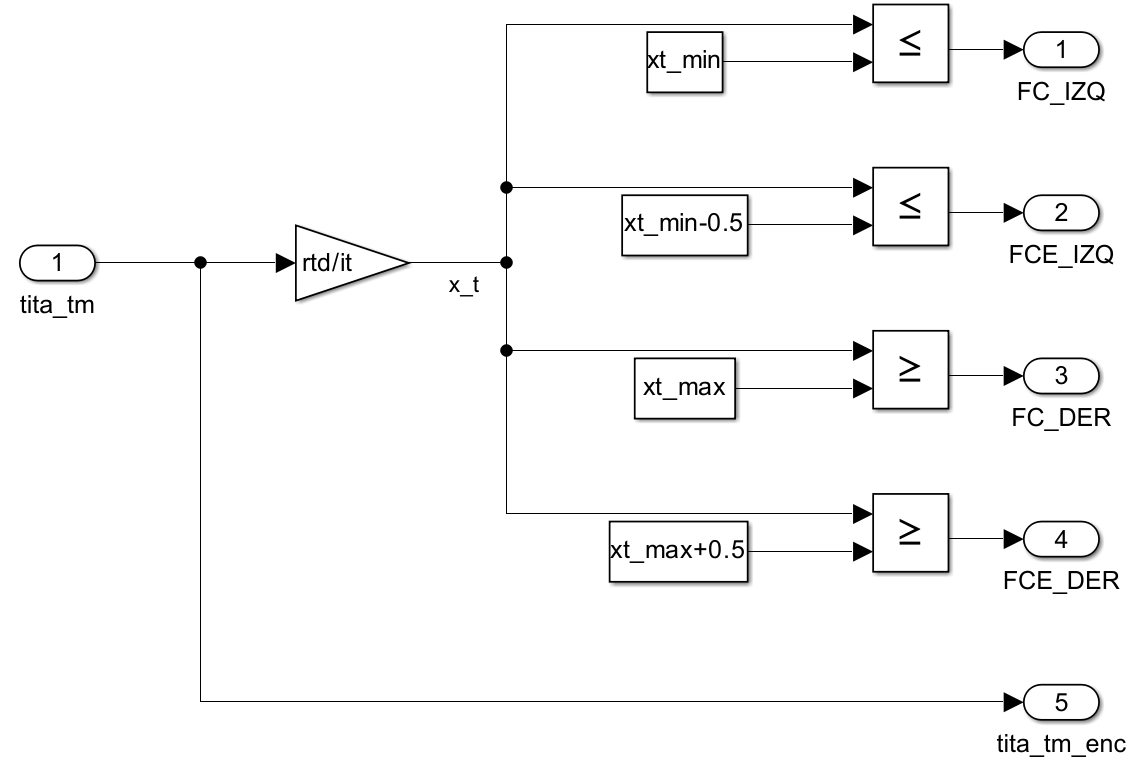
\includegraphics[width=\textwidth]{sensores_carro.png}
      \caption{Diagrama de bloques sensores carro e izaje Simulink}
      \end{figure}
    \end{column}
    \begin{column}{0.48\textwidth}
      \centering
      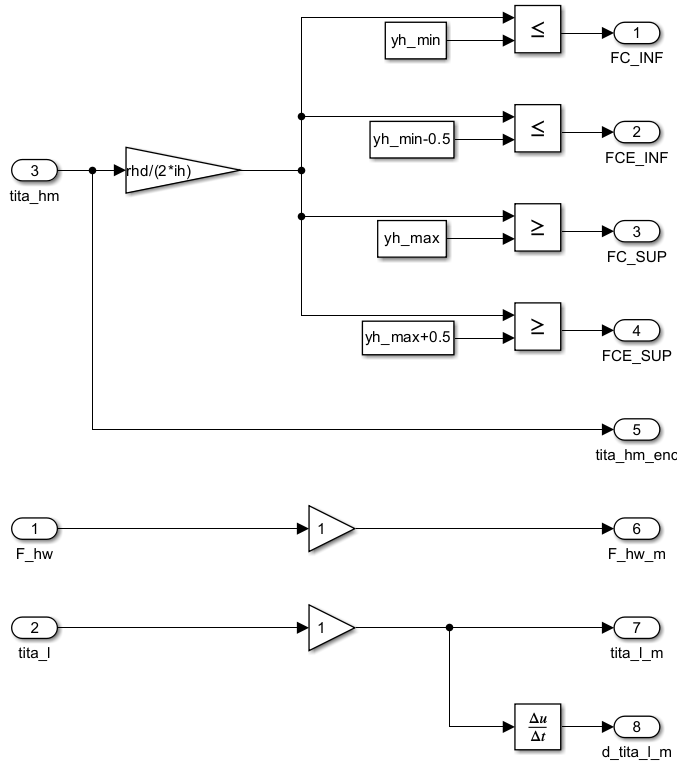
\includegraphics[width=\textwidth]{sensores_izaje.png}
    \end{column}
  \end{columns}
\end{frame}


\begin{frame}{Moduladores de torque}
  \begin{block}{Función en la simulación}
    Modelan las limitaciones de los \textbf{accionamientos reales} (motores eléctricos)
    \begin{itemize}
      \item No es posible aplicar torque instantáneo como una fuerza mecánica ideal
      \item Los motores reales tienen capacidad limitada y retardo dinámico
    \end{itemize}
  \end{block}

  \begin{block}{Dos funciones clave}
    \begin{enumerate}
      \item \textbf{Saturación}: limita torque a máximo permitido $T_{\max}$
      \item \textbf{Filtrado}: modela retardo electromagnético con constante $\tau = 1$ ms
    \end{enumerate}
  \end{block}
  \begin{block}{Ecuación diferencial}
    Vincula el torque limitado comandado $T_{\text{Lim}}^*(t)$ con el torque físico real $T(t)$:
    \vspace{-0.2cm}
    \[
    \tau \frac{dT(t)}{dt} = T_{\text{Lim}}^*(t) - T(t)
    \]
  \end{block}

\end{frame}


\begin{frame}{Modulador del carro}
  \begin{block}{Ecuación}
    \[
T_{tm\ Lim}^*(k \, T_{s2} \leq t < (k+1) \, T_{s2}) = \text{min}\left(+T_{tm\max}, \text{max}\left(-T_{tm\max}, T_{tm}^*(k \, T_{s2})\right)\right)
    \]
  \end{block}
  \begin{figure}
  \centering
  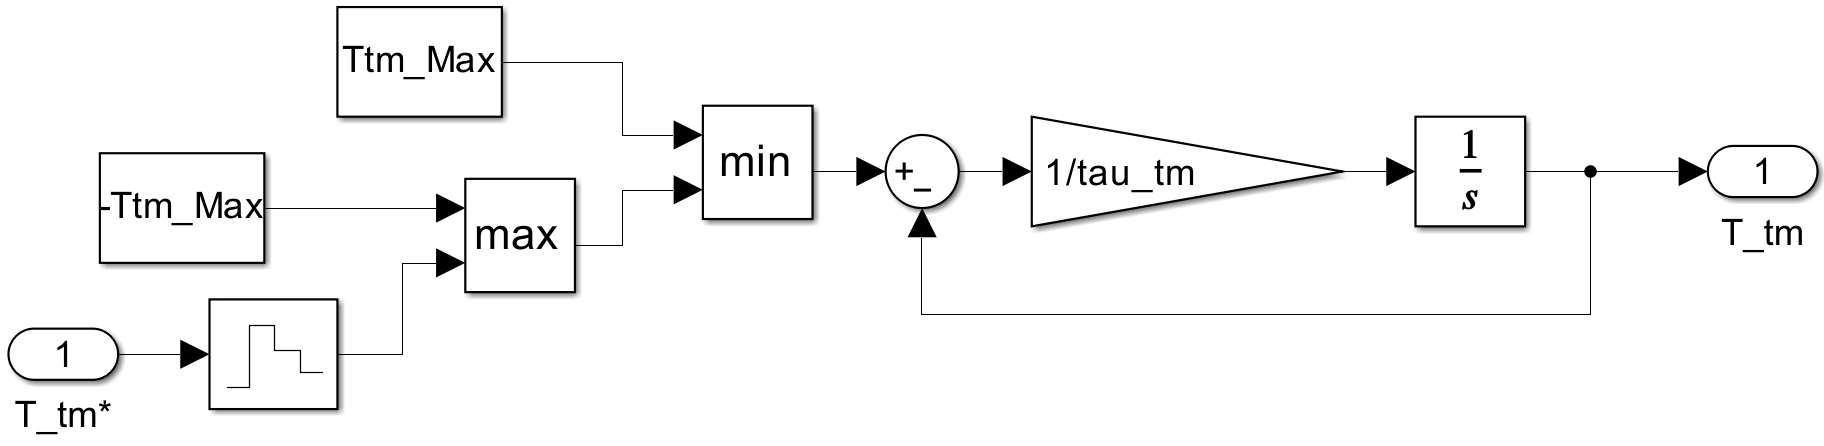
\includegraphics[width=1\textwidth]{modulador_carro.png}
  \caption{Diagrama de bloques del modulador de torque del carro}
  \end{figure}
\end{frame}
